
\chapter{Materiais e Métodos}

\subsection{Correção de mapas de profundidade} 

Para a tarefa de correção de mapas de profundidade utilizando redes neurais, o trabalho de \cite{hu2022deep} propôs duas categorias principais que se diferenciam pelos dados utilizados:

\begin{itemize}
    \item \textbf{Correção não-guiada} (Figura \ref{ung}): Objetiva completar diretamente as partes faltantes utilizando como entrada somente o mapa de profundidade.
    \item \textbf{Correção guiada} (Figura \ref{early} e \ref{late}): Objetiva completar as partes faltantes utilizando como entrada tanto o mapa de profundidade quanto a imagem RGB correspondente.
\end{itemize}

\begin{figure}[h]
    \centering
    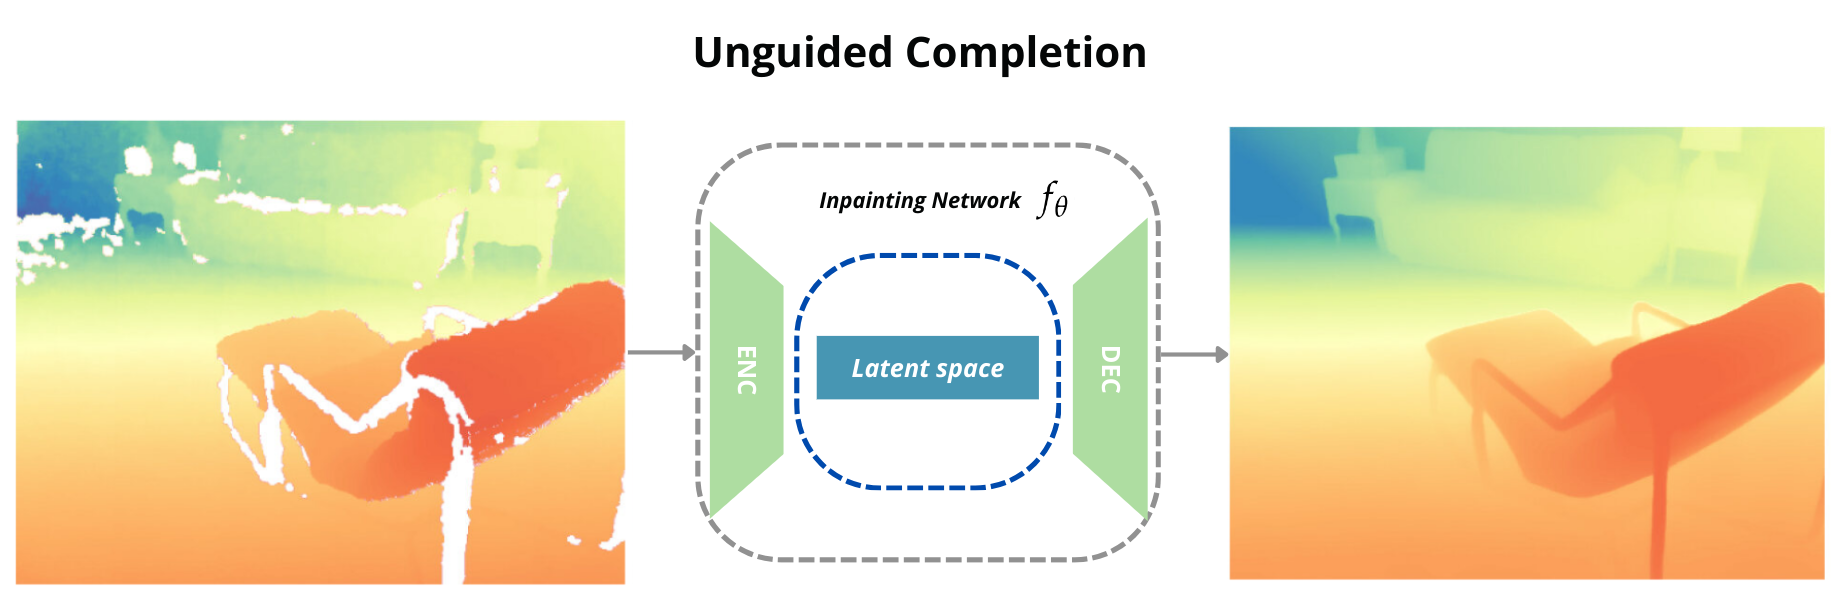
\includegraphics[width=\textwidth]{fig/unguided.png}
    \caption{Esquema de correção não-guiada.}
    \label{ung}
\end{figure}

A escolha da categoria de correção depende da quantidade de erros nas imagens. Quando há uma pequena quantidade de pixels inválidos, a correção não-guiada pode ser adequada, visto que não é necessário uma profunda extração de características dos dados. No entanto, no caso contrário, o uso de métodos guiados é indicado dado que existam grandes regiões com ausência de informação de profundidade ou que o mapa apresente uma grande esparsidade. Sendo necessário recorrer a extração dos atributos presentes na imagem RGB como bordas, contornos, estruturas de objetos não identificados pelo sensor e característica de descontinuidade de superfícies \cite{hu2022deep}.

Ainda no trabalho de \cite{hu2022deep}, nomeia-se outras subcategorias de técnicas de correção guiada. Uma delas é chamada de \textit{Early Fusion} (Figura \ref{early}) e consiste em utilizar a imagem RGB concatenada ao mapa de profundidade com erros como entrada da rede neural. Essa técnica possui a vantagem de ser simples e de baixa complexidade. A outra, conhecida como \textit{Late Fusion} (Figura \ref{late}) envolve transferir a fusão da imagem RGB com o mapa em ramos distintos da rede neural, chamados \textit{RGB Encoder-Decoder} e \textit{Depth Encoder-Decoder}.

\begin{figure}[h]
    \centering
    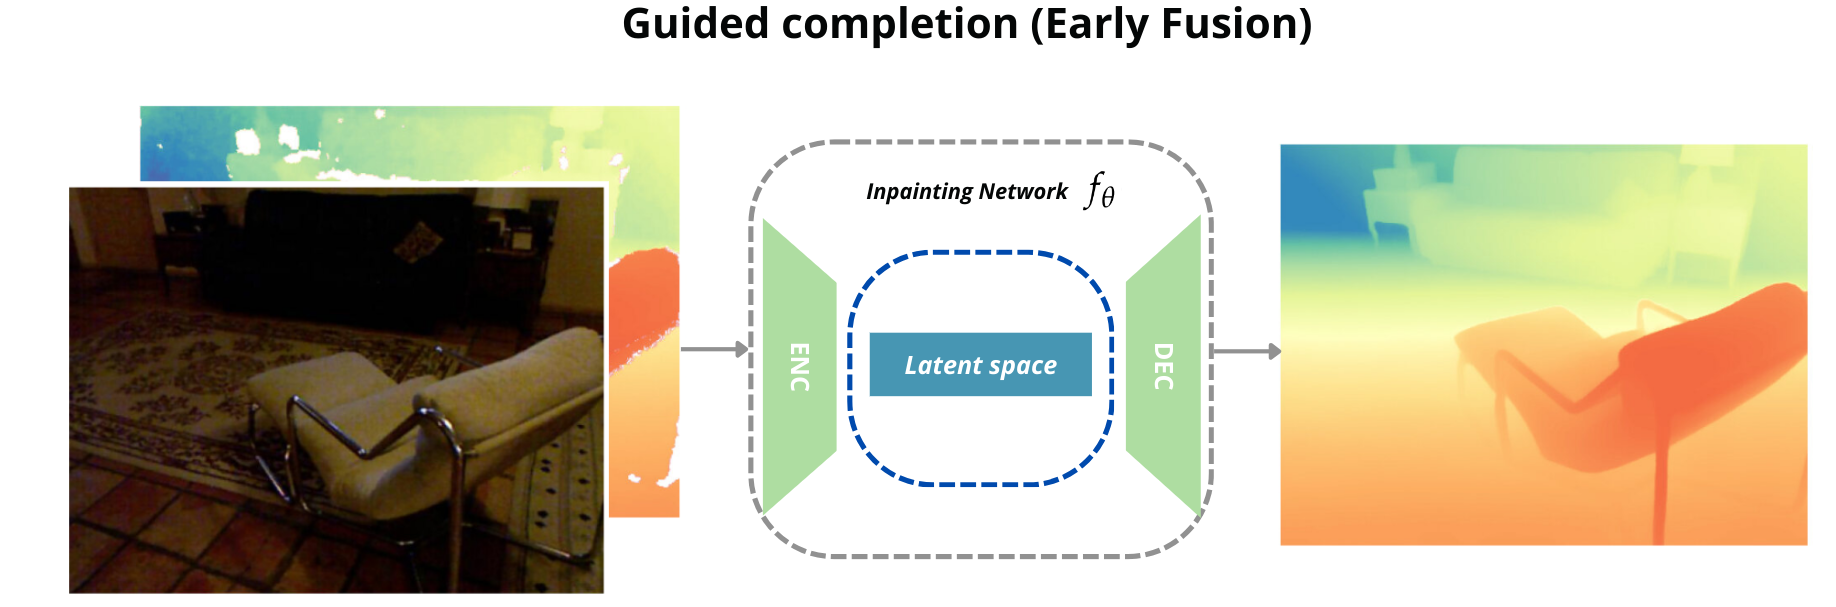
\includegraphics[width=\textwidth]{fig/earlyfusion.png}
    \caption{Esquema de correção guiada com \textit{Early Fusion}.}
    \label{early}
\end{figure}

\begin{figure}[h]
    \centering
    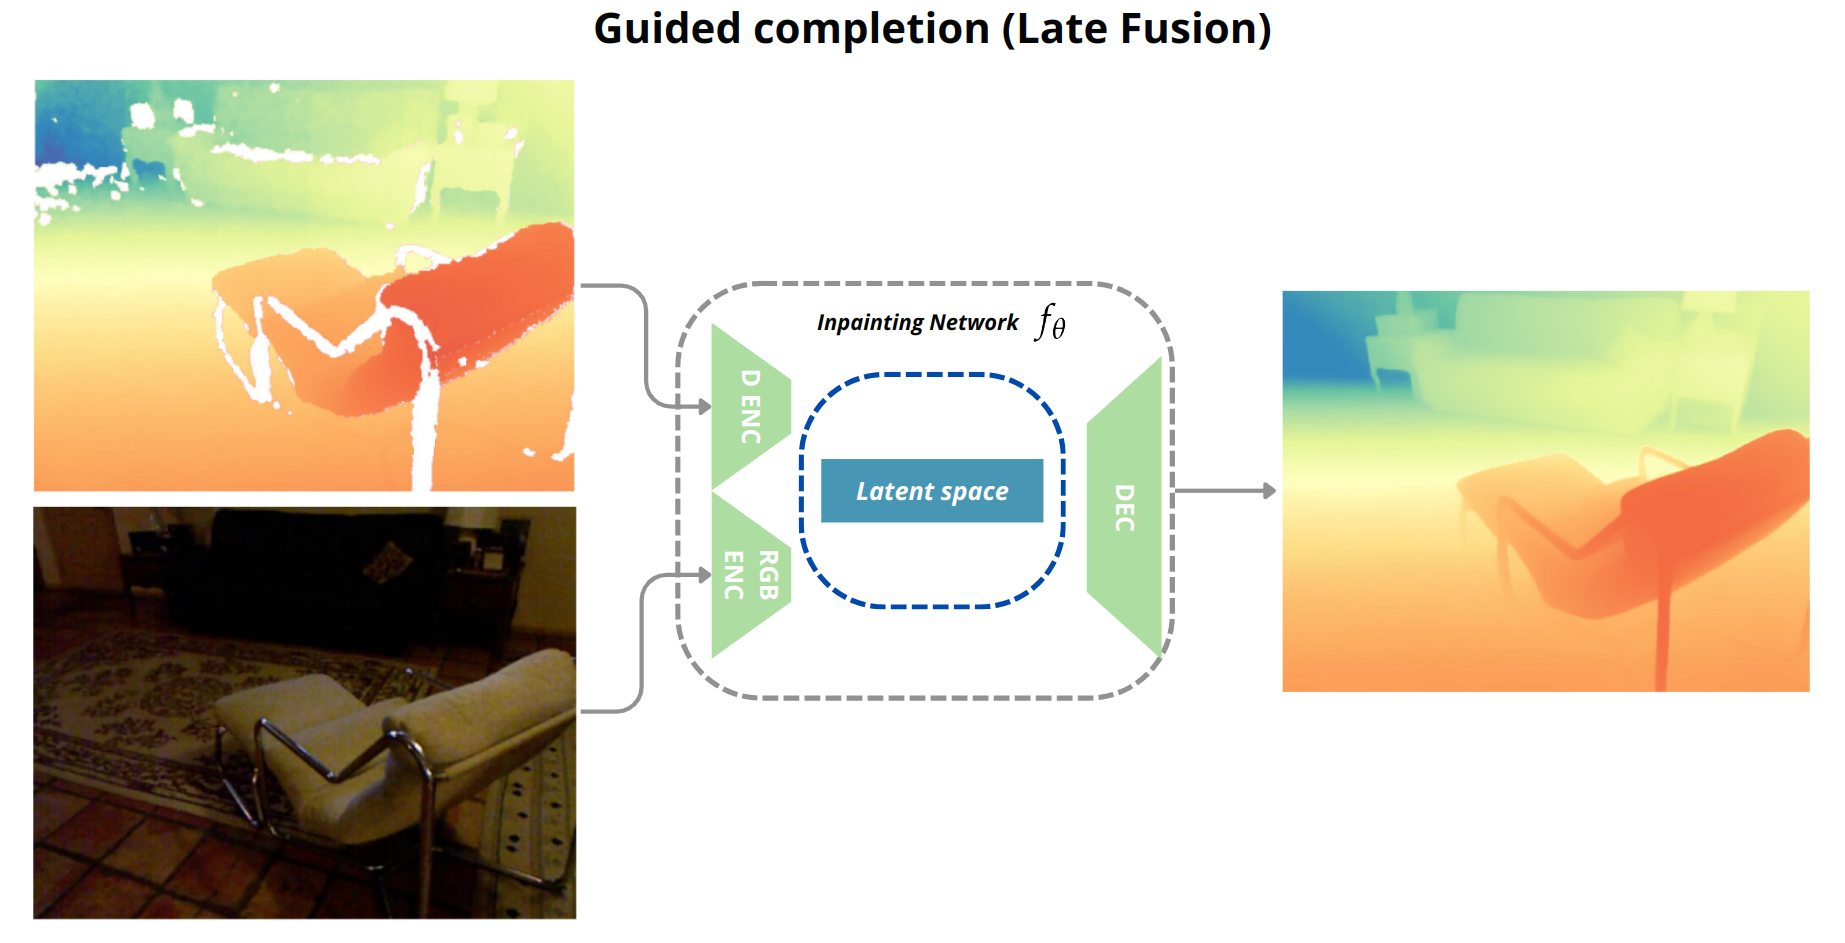
\includegraphics[width=\textwidth]{fig/latefusion.png}
    \caption{Esquema de correção guiada com \textit{Late Fusion}.}
    \label{late}
\end{figure}


\subsection{Large Mask Inpainting}

%Image inpainting is the process of completing or recovering the missing region in the image or removing some objects added to it. 

\textit{Image Inpainting} refere-se ao processo de recuperar regiões faltantes de uma imagem a partir de informação já existente \cite{elharrouss2020image}. Para sintetizar as partes indicadas, é necessário que haja o aprendizado da estrutura global da imagem, sendo imprescindível um vasto campo receptivo na rede neural. Dessa forma, é proposto por \cite{suvorov2022resolution} o sistema LaMa, \textit{Large Mask Inpainting} (Figura \ref{lama}), que é composto por elementos capazes de explorar o campo receptivo apropriado para essa tarefa, sendo eles: i) convoluções rápidas de Fourier (do inglês, \textit{Fast Fourier Convolutions}), ii) o uso de perda perceptual baseada em uma rede de segmentação e iii) uma estratégia de geração de máscaras para treinamento de alta cobertura.

\begin{figure}[h]
    \centering
    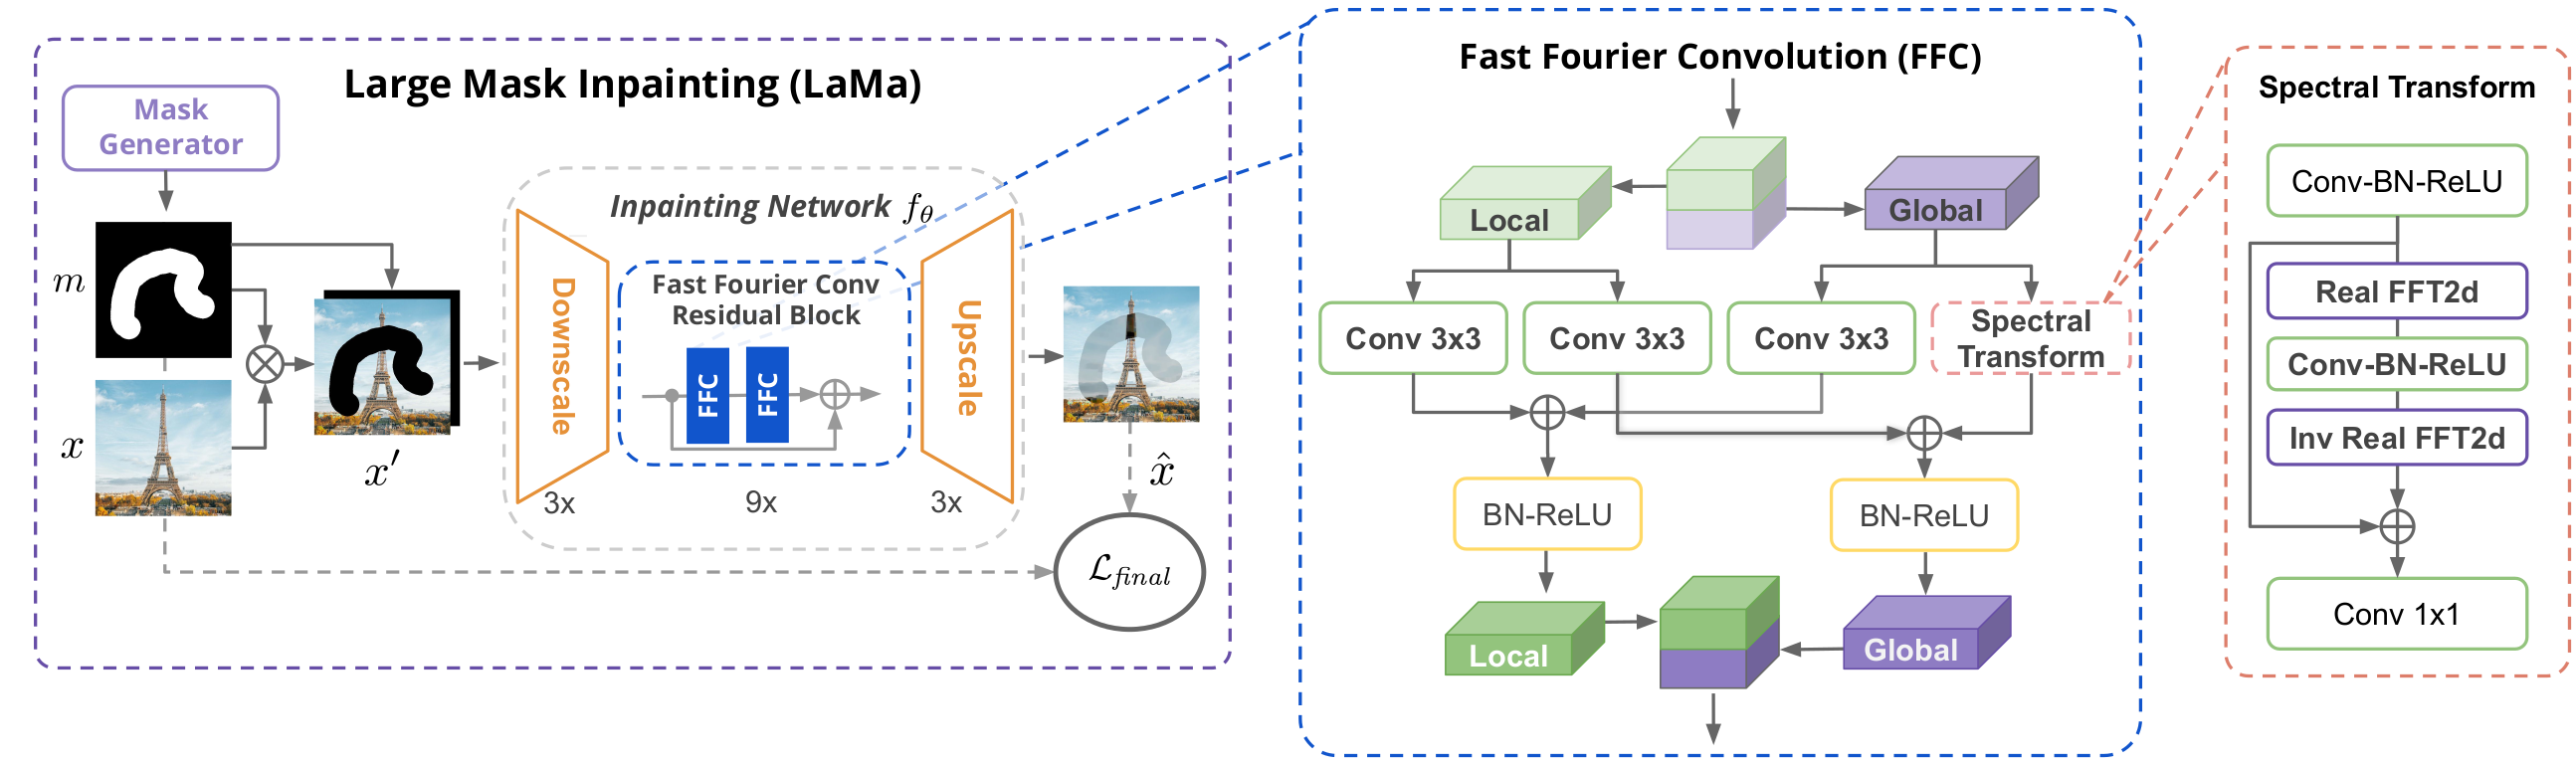
\includegraphics[width=\textwidth]{fig/lama.png}
    \caption{Esquema do método LaMa \cite{suvorov2022resolution}.}
    \label{lama}
\end{figure}

%explain receptive field?

\section{Datasets}

O presente trabalho exige um tipo de base de dados pouco encontrado na literatura, trios de imagem RGB, mapa de profundidade com erros e um outro mapa de profundidade denso e completo. De acordo com \cite{zhang2018deep}, uma das maneiras de se obter esses dados seria capturar imagens com uma câmera RGB-D de baixo custo e alinha-las com outra captura simultânea de um sensor mais preciso, porém essa abordagem é muito custosa, além de que não há disponibilidade de grandes conjuntos para treinamento.

O presente projeto pretende utilizar como base de dados principal o \textbf{Hypersim}. Um \textit{dataset} para compreensão de cenas baseado em cenas sintéticas fotorrealistas. Contendo 77.400 imagens de 461 cenas \textit{indoor} com pares de RGB e mapas de profundidade calculado deterministicamente, além de outras informações como normais de superfície, rótulos de segmentação e detecção de objetos e entre outros \cite{roberts2021hypersim}.

\section{Metodologia da Pesquisa}





